\chapterauthor{Krzysztof Szostak}
\chapter[Kaskadowy model \ldots]{Kaskadowy model obwodowy w metodach pomiaru parametrów elektrycznych cienkich podłoży dielektrycznych}
\thispagestyle{empty}
\vspace{-8mm} {\large Krzysztof Szostak} \vspace{8mm}

\section{Wprowadzenie}
Współczesna telekomunikacja wykorzystuje przede wszystkim planarne obwody mikrofalowe zbudowane na bazie podłoży w postaci cienkich laminatów lub ceramik. Dokładna znajomość parametrów elektrycznych oraz zmienności tych parametrów w obrębie badanego podłoża jest niezwykle ważna ze względu na prawidłowe działanie oraz wydajność wykonanego na ich podstawie układu wysokiej częstotliwości. Ma to szczególne znaczenie w przypadku obwodów pracujących w paśmie EHF (\textit{ang. Extremely High Frequency}) o bardzo małych wymiarach geometrycznych.
\par Istnieje wiele rezonansowych \cite{cite:res1,cite:res2} i nierezonansowych \cite{cite:nonres1,cite:nonres2}  metod pomiaru przenikalności elektrycznej materiałów dielektrycznych w postaci cienkich podłoży. Metody rezonansowe charakteryzują się wysoką czułością, ale umożliwiają pomiar jedynie w wąskim zakresie częstotliwości, np. metoda SPDR (\textit{ang. Split Post Dielectric Resonator}) \cite{cite:SPDR}. Z kolei metody nierezonansowe są mniej czułe od metod rezonansowych. Pozwalają jednak na szerokopasmową obserwację parametrów elektrycznych badanego materiału.
\par W niniejszym opracowaniu przedstawiono dwie szerokopasmowe metody pomiaru parametrów elektrycznych podłoża dielektrycznego wykorzystujące planarne obwody mikrofalowe, tj. metodę różnicowej fazy \cite{cite:two_lines_method} będącej standardem przemysłowym oraz metodę zmiany szerokości linii mikropaskowej \cite{cite:line_width_method}. Największy nacisk położono na omówienie zasady działania metody zmiany szerokości linii mikropaskowej wraz z opisem użytej macierzy łańcuchowej. Ma to na celu przedstawienie głównych kroków umożliwiających wyprowadzenie równania analitycznego (patrz sekcja \ref{sec:numerical}) pozwalającego na obliczenie śladu macierzy wynikowej. Jest to znaczące rozwinięcie algorytmu numerycznego zaproponowanego w \cite{cite:line_width_method} i opisanego szerzej w \cite{cite:doktorat}.

\section{Metoda różnicowej fazy}

Metoda różnicowej fazy (dwóch linii) \cite{cite:two_lines_method} polega na wykonaniu dwóch pomiarów parametrów $S$ krótszej $l_2$ i dłuższej linii mikropaskowej $l_1$ znajdujących się w~niewielkiej odległości od siebie na tym samym obszarze badanego podłoża dielektrycznego (rys. \ref{fig:phase_difference_method_main} \cite{cite:doktorat}). W innej wersji metody różnicę długości otrzymuje się poprzez obcięcie fragmentu podłoża i ponowne osadzenie złącza pomiarowego (rys. \ref{phase_diff_method_effective_permittivity_eq} \cite{cite:doktorat}). Krótszą i dłuższą linię mikropaskową mierzy się z wykorzystaniem wektorowego analizatora sieci i na podstawie parametru $S_{21}$ odczytuje się różnicę opóźnienia fazowego $\Delta\phi$ pomiędzy obiema liniami transmisyjnymi przy danej częstotliwości $f$. Efektywna stała dielektryczna podłoża jest powiązana ze zmierzoną różnicą fazy następującym wyrażeniem \cite{cite:two_lines_method}:

 \begin{equation}
        \Delta\phi = 2\pi f\frac{\sqrt{\varepsilon_{eff}}}{c}\Delta l \text{,}
 \end{equation}
 
\noindent gdzie $c$ to prędkość światła w próżni, a $\Delta l$ to różnica długości obu linii. Po przekształceniu otrzymuje się zależność:

 \begin{equation}
\label{phase_diff_method_effective_permittivity_eq}
 \varepsilon_{eff} = \left( \frac{\Delta \phi \: c}{2 \pi f \Delta l} \right) ^2 \text{.}
 \end{equation}

Istnieje również wersja metody różnicowej fazy wykorzystująca ślad macierzy \cite{cite:two_lines_method_trace}. Dzięki temu zabiegowi uzyskuje się odporność na niedopasowanie impedancyjne we wrotach linii mikropaskowej. Oczywistym problemem metody dwóch linii jest konieczność modyfikacji podłoża oraz błąd związany z mocowaniem złącz pomiarowych. Wymaga się także, aby różnica długości wykorzystanych linii transmisyjnych była jak największa.

 \begin{figure}[tbh!]
    \centering{\includesvg[inkscapelatex=false,width=0.6\columnwidth]{fig/ch3/ch3_phase_difference_method_main}}
    \caption{Metoda różnicowej fazy – wersja z dłuższym i krótszym odcinkiem linii mikropaskowej wykonanej na tym samym obszarze badanego podłoża dielektrycznego.}
\label{fig:phase_difference_method_main}
\end{figure}

  \begin{figure}[tbh!]
    \centerline{\includesvg[inkscapelatex=false,width=0.6\columnwidth]{fig/ch3/phase_difference_method_other}}
    \caption{Metoda różnicowej fazy – wersja z przycinanym podłożem dielektrycznym.}
\label{fig:phase_difference_method_other}
\end{figure}

\section[Metoda z linią mikropask. o zmiennej szer.]{Metoda z linią mikropaskową o zmiennej szerokości}

Odpowiedzią na zasygnalizowane wcześniej problemy w metodzie różnicowej fazy może być współopracowana przez autora metoda oparta na zmianie szerokości linii mikropaskowej \cite{cite:line_width_method} polegająca na użyciu pojedynczej linii mikropaskowej zawierającej symetryczną nieciągłość skokową (rys. \ref{fig:microstripe_width_change_schematic} \cite{cite:doktorat}). Metoda wymaga przeprowadzenia dwóch następujących po sobie pomiarów parametrów $S$ linii mikropaskowej przed i po modyfikacji szerokości środkowego segmentu linii. Kolejność modyfikacji jest dowolna i zależy od wybranej metody nakładania metalizacji. W efekcie nie ingeruje się w raz przymocowane złącza pomiarowe i~geometrię podłoża.
\par Ekstrakcja stałej dielektrycznej po wykonaniu pomiarów przed i po modyfikacji segmentu linii polega na wykorzystaniu dwóch modeli kaskadowych linii transmisyjnej z nieciągłościami i bez nich (przy założeniu, że przed lub po modyfikacji otrzymuje się typową linię mikropaskową) oraz na zamianie parametrów rozproszenia $S$ na transmisyjną macierz $T (ABCD)$. Na rys. \ref{fig:testbench} \cite{cite:doktorat} przedstawiono rzeczywiste stanowisko pomiarowe do badania stałej dielektrycznej podłoża metodą ze zmianą szerokości linii mikropaskowej (wymiary linii: $h$~=~1,524~mm, $t$~=~18~$\mu \text{m}$, $w_1$ = 5,8 mm, $w_2$ = 1,8 mm, $l_c$~=~25~mm, $l$ = 50 mm).

\begin{figure}[tbh]
   \centerline{\includesvg[inkscapelatex=false,width=0.6\columnwidth]{fig/ch3/microstripe_width_change_schematic}}
    \caption{Metoda z linią mikropaskową o zmiennej szerokości: geometria linii mikropaskowej przed modyfikacją  (na górze); geometria linii mikropaskowej po modyfikacji (na dole).}
\label{fig:microstripe_width_change_schematic}
\end{figure}

\begin{figure}[b!]
     \centering
     \begin{subfigure}{0.49\textwidth}
         \centering
         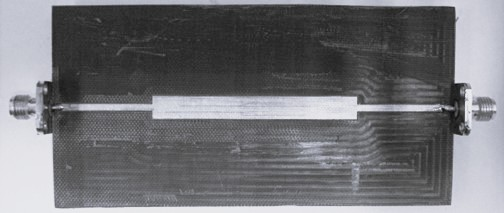
\includegraphics[width=\textwidth]{fig/ch3/microstripe_width_change_real_measurement.jpg}
         
         \caption{}
         \label{fig:microstripe_width_change_real_measurement_wide}
     \end{subfigure}
     \hfill
     \begin{subfigure}{0.44\textwidth}
         \centering
         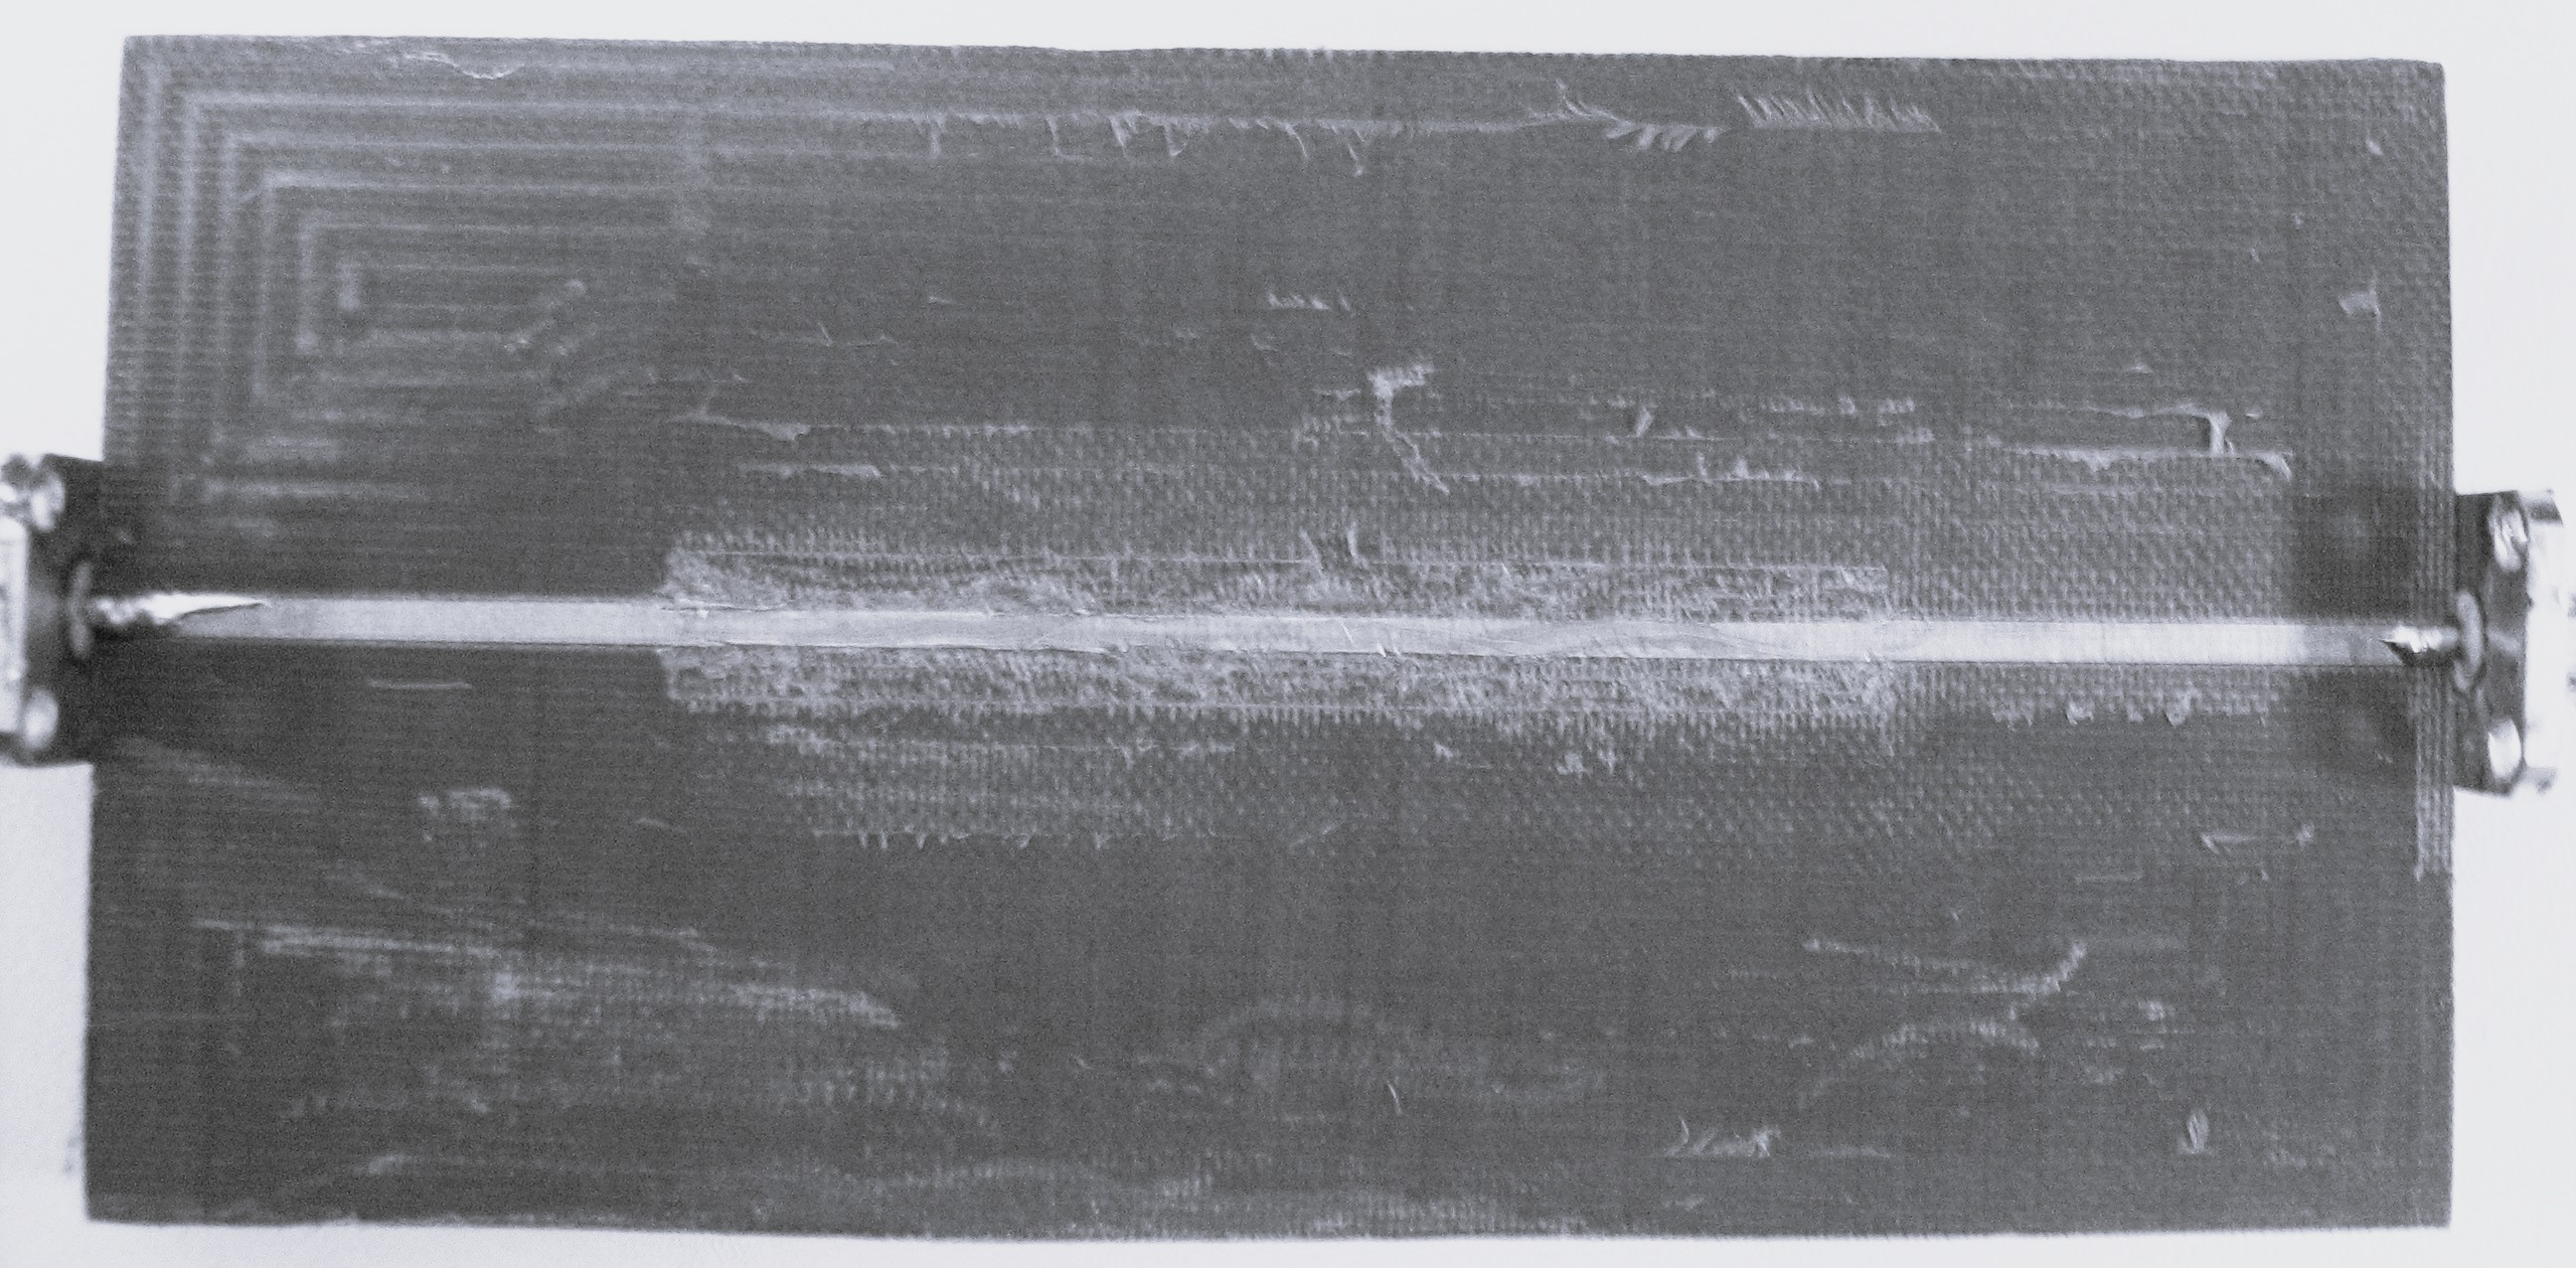
\includegraphics[width=\textwidth]{fig/ch3/microstripe_width_change_real_measurement_thin.jpg}
         
         \caption{}
         \label{fig:microstripe_width_change_real_measurement_thin}
     \end{subfigure}
     \hfill
     \begin{subfigure}{0.35\textwidth}
         \centering
         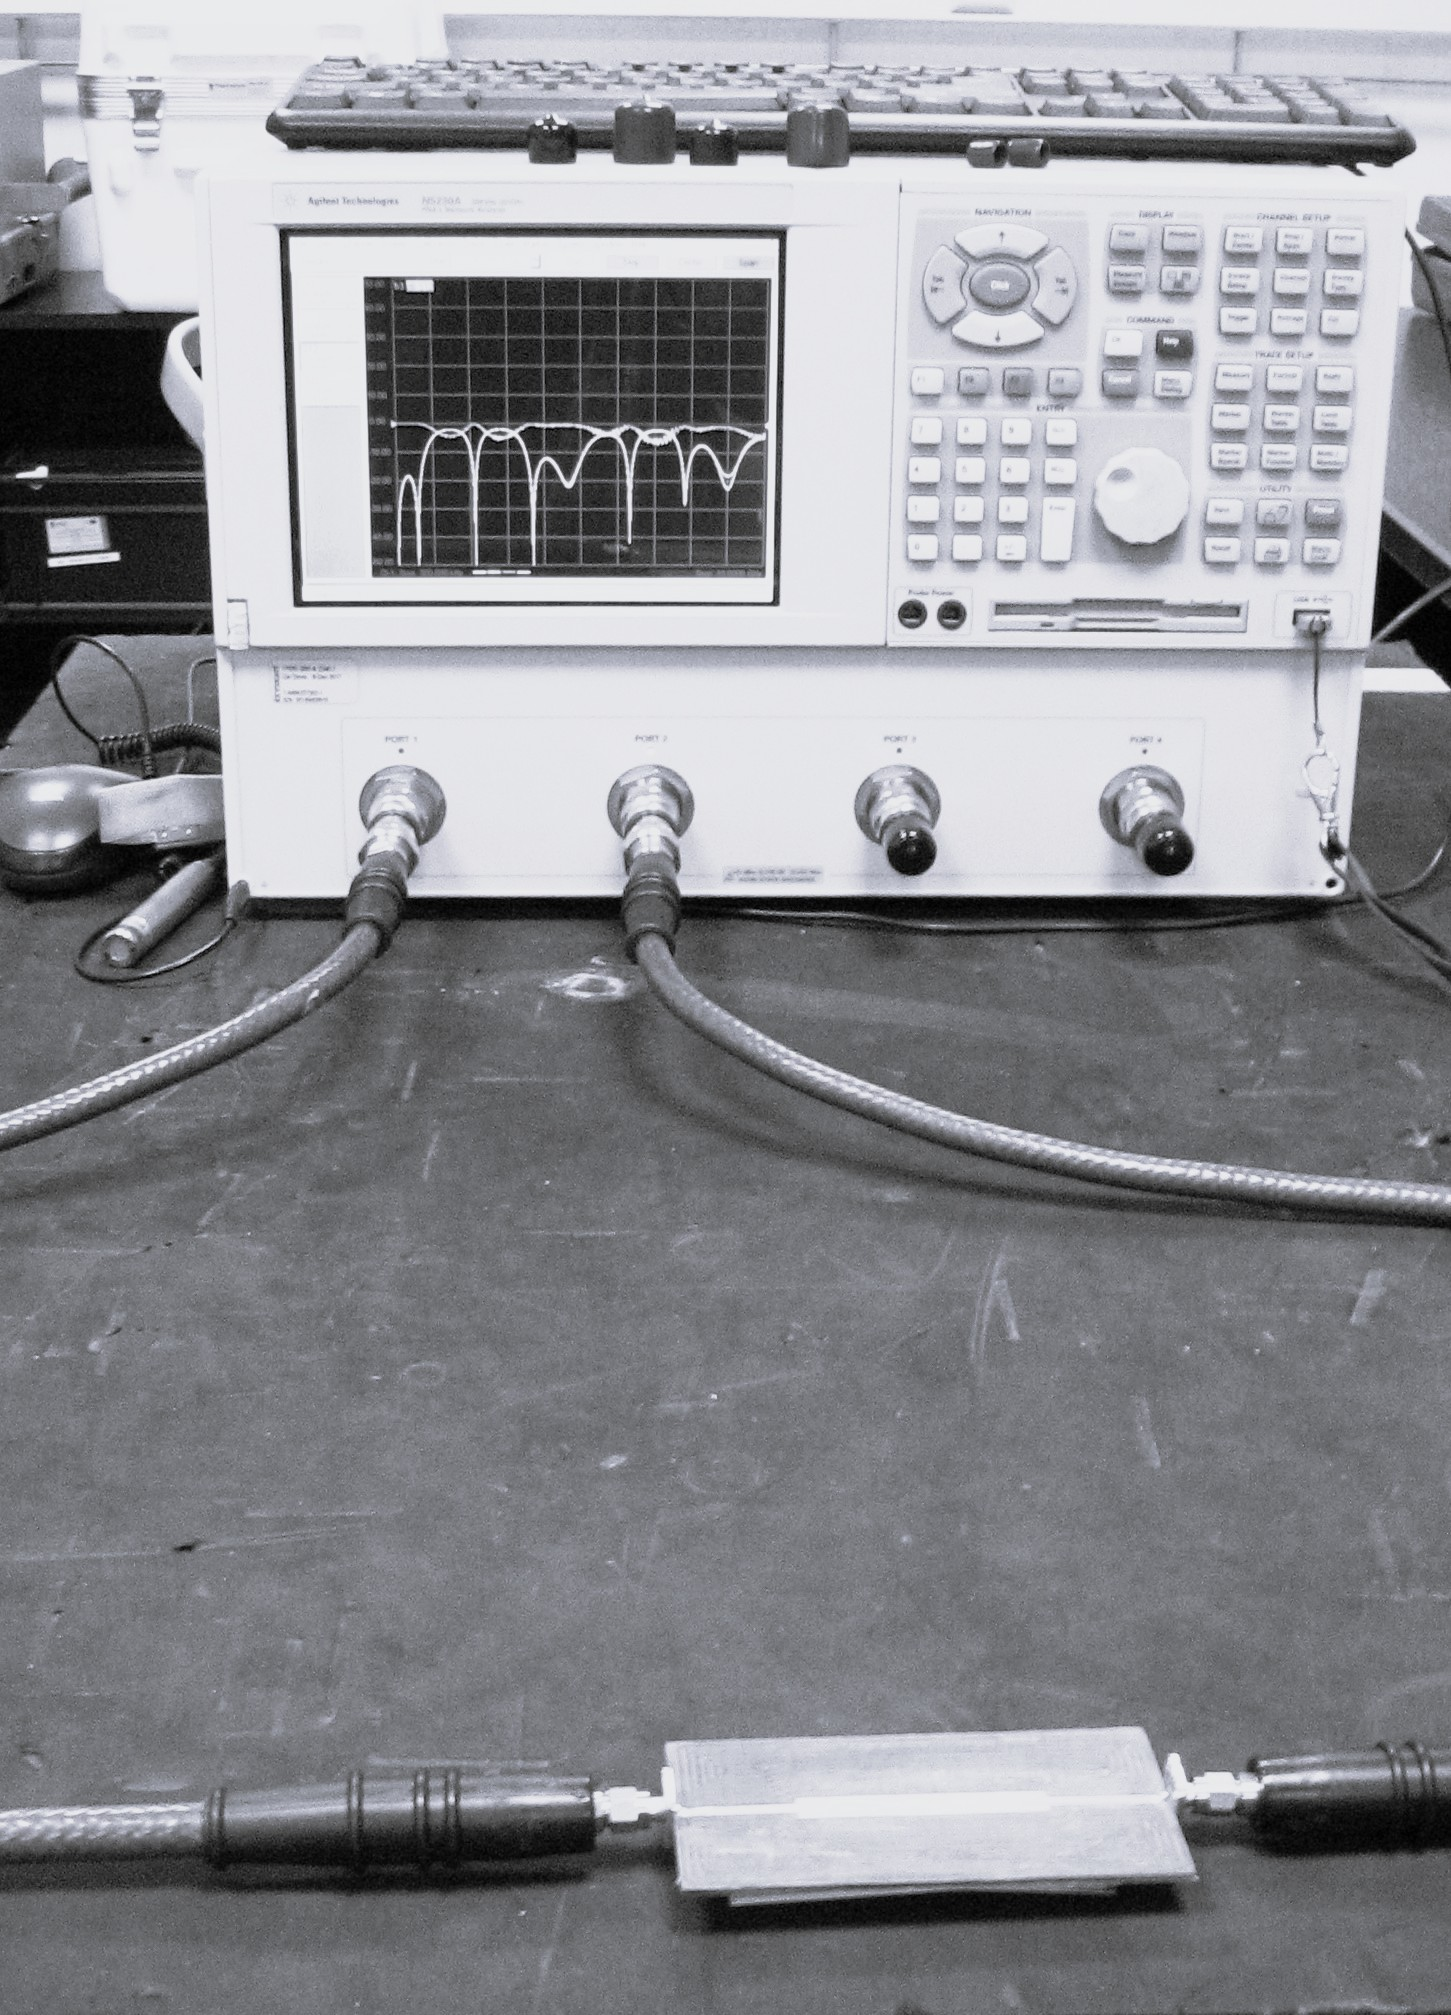
\includegraphics[width=1\textwidth]{fig/ch3/microstrip_width_change_testbench}
         
         \caption{}
         \label{fig:microstripe_width_change_real_measurement_testbench}
     \end{subfigure}
     
     \caption{Transmisyjna linia mikropaskowa zbudowana na laminacie mikrofalowym Rogers Ultralam 2000: a) przed modyfikacją b) po modyfikacji c) stanowisko pomiarowe.} \label{fig:testbench}
\end{figure}

\subsection{Model kaskadowy}

W dalszych rozważaniach przyjęto, że modyfikacja środkowego segmentu linii polega na jego zwężeniu. Model kaskady z symetryczną nieciągłością skokową przedstawiono na rys. \ref{fig:microstripe_width_change_cascade_t1} \cite{cite:doktorat} i składa się on z następujących elementów reprezentowanych przez macierze łańcuchowe: lewostronne złącze SMA ($T_{CL}$), lewostronną węższą linię mikropaskową ($T_{lc}$) o szer. $w_2$ i dł. $l_c$, lewostronną nieciągłość skokową ($T_{SL}$), szeroką linię mikropaskową ($T_{L1}$) o szer. $w_1$ i dł. $l$ tworzącą środkowy segment linii mikropaskowej, prawostronną nieciągłość skokową ($T_{SR}$), prawostronną węższą linię mikropaskową ($T_{lc}$) o szer. $w_2$ i dł. $l_c$ oraz prawostronne złącze SMA ($T_{CR}$). Z kolei model bez nieciągłości skokowej (rys. \ref{fig:microstripe_width_change_cascade_t2} \cite{cite:doktorat}) składa się z lewostronnego złącza SMA ($T_{CL}$), lewostronnej węższej linii mikropaskowej ($T_{lc}$) o szer. $w_2$ i dł. $l_c$, wąskiej linii mikropaskowej ($T_{L1}$) o~szer. $w_2$ i dł. $l$ tworzącą środkowy segment linii mikropaskowej, prawostronnej węższej linii mikropaskowej ($T_{lc}$) o szer. $w_2$ i dł. $l_c$ oraz prawostronnego złącza SMA ($T_{CR}$).

Procedurę ekstrakcji stałej dielektrycznej rozpoczyna się od sytuacji przedstawionej na rys. \ref{fig:microstripe_width_change_cascade_t1} (przed modyfikacją), którą opisuje poniższe równanie \cite{cite:two_lines_method_trace}:

\begin{figure}[tbh!]
     \centering
     \begin{subfigure}[b]{1\textwidth}
         \centering
         %\hspace*{-0.15\textwidth}
         {\includesvg[inkscapelatex=false,width=1\textwidth]{fig/ch3/cascade_t1}
         \caption{}
         \label{fig:microstripe_width_change_cascade_t1}}
     \end{subfigure}
     \hfill
     \begin{subfigure}[b]{1\textwidth}
         \centering
         {\includesvg[inkscapelatex=false,width=1\textwidth]{fig/ch3/cascade_t2}}
         \caption{}
         \label{fig:microstripe_width_change_cascade_t2}
     \end{subfigure}
        \caption{Kaskada dwuwrotników opisanych za pomocą macierzy łańcuchowych dla układu z rys.~\ref{fig:microstripe_width_change_schematic}: a)~przed modyfikacją b) po modyfikacji}
        \label{fig:microstripe_width_change_cascade}
\end{figure}

 \begin{equation}
    \label{cascade_main_eq}
      T=T_L\cdot T_{SL}\cdot T_{L1}\cdot T_{SR}\cdot T_R \text{,}
 \end{equation}

\noindent przy czym:

\begin{equation}
    \label{cascade_main_1_eq}
      T_L = T_{CL} \cdot T_{lc} \text{,}
 \end{equation}

    \begin{equation}
    \label{cascade_main_2_eq}
      T_R = T_{lc} \cdot T_{CR} \text{.}
 \end{equation}

 \noindent Kluczowym uproszczeniem i głównym źródłem błędu przedstawionej metody jest założenie równości obu nieciągłości skokowych, co umożliwia wprowadzenie następujących założeń \cite{cite:two_lines_method_trace}:

    \begin{equation}
    \label{cascade_main_3_eq}
      T_{SL} = T_{SR} =T_{S} \text{.}
 \end{equation}

 \noindent W efekcie otrzymujemy poniższe zależności opisujące linię mikropaskową przed i po modyfikacji środkowego segmentu: 

  \begin{equation}
    \label{cascade_main_extended_eq}
      T_1=T_L\cdot T_{S}\cdot T_{L1}\cdot T_{S}\cdot T_R \text{,}
 \end{equation}

    \begin{equation}
    \label{cascade_main_extended_after_modification_eq}
      T_2=T_{L} \cdot T_{L2} \cdot T_{R} \text{.}
 \end{equation}

\noindent Przeprowadzając operację mnożenia macierzy otrzymuje się poniższe równanie:

   \begin{equation}
    \label{cascade_main_extended_2_eq}
     T_2^{-1}T_1=T_R^{-1}T_{L2}^{-1}T_L^{-1}\cdot T_LT_ST_{L1}T_S T_R = T_R^{-1}T_{L2}^{-1} \cdot T_ST_{L1}T_S T_R \text{,}
 \end{equation}

\noindent a korzystając z właściwości śladu macierzy dostajemy następującą zależność:

   \begin{equation}
    \label{cascade_main_extended_3_eq}
      TR=Tr\left(T_2^{-1}T_1\right)\ =Tr\left(T_{L2}^{-1}T_ST_{L1}T_S\right)=Tr\left(T_{M2}^{-1}T_{M1}\right) \text{,}
 \end{equation}

\noindent przy czym:

   \begin{equation}
    \label{cascade_main_extended_4_eq}
      T_{M1}=T_ST_{L1}T_S,
 \end{equation}

    \begin{equation}
    \label{cascade_main_extended_5_eq}
      T_{M2}=T_{L2} \text{.}
 \end{equation}

 \noindent Każdy z elementów składowych kaskady (\ref{cascade_main_extended_3_eq}) jest zależny od mierzonej stałej dielektrycznej podłoża \cite{cite:doktorat}:

  \begin{align}
   \begin{split}
    \label{cascade_main_epsilon_dependant_eq}
      TR \left( \varepsilon_r \right)&=
      Tr\left(T_2^{-1}\left( \varepsilon_r \right)T_1\left( \varepsilon_r \right)\right)\ = \\
  &=Tr\left(T_{M2}^{-1}\left( \varepsilon_r \right)T_{M1}\left( \varepsilon_r \right)\right)= \\
        &=Tr\left(T_{L2}^{-1}\left( \varepsilon_r \right)T_S\left( \varepsilon_r \right)T_{L1}\left( \varepsilon_r \right)T_S\left( \varepsilon_r \right)\right) \text{.}
 \end{split}    
 \end{align}




\subsection{Macierze łańcuchowe}

Model numeryczny wykorzystany w metodzie ze zmianą szerokości linii mikropaskowej wykorzystuje transmisyjną macierz ABCD linii mikropaskowej przedstawioną poniżej \cite{cite:microstrip_book}:

  \begin{figure}[tbh!]
     \centering
     \begin{subfigure}[b]{0.49\textwidth}
         \centering
         %\hspace*{-0.15\textwidth}
         {\includesvg[inkscapelatex=false,width=0.6\columnwidth]{fig/ch3/step_discontinuity_physical}}
         \caption{}
         \label{fig:step_discontinuity_physical}
     \end{subfigure}
     \hfill
     \begin{subfigure}[b]{0.49\textwidth}
         \centering
         {\includesvg[inkscapelatex=false,width=0.6\columnwidth]{fig/ch3//step_discontinuity_schematic}}
         \caption{}
         \label{fig:step_discontinuity_schematic}
     \end{subfigure}
        \caption{Mikropaskowa nieciągłość skokowa: a) reprezentacja fizyczna
b) model obwodowy.}
        \label{fig:step_discontinuity}
\end{figure}



\begin{equation}
    \label{microstrip_T_matrix_general_eq}
     T= \begin{bmatrix}
          \cos{\left( \gamma_c L \right)} & j \cdot Z_c\sin{\left( \gamma_c L \right)} \\
          j \cdot \cfrac{1}{Z_c} \sin{\left( \gamma_c L \right)} & \cos{\left( \gamma_c L \right)}
      \end{bmatrix} \text{,}
 \end{equation}

 \noindent gdzie $L$ to długość linii mikropaskowej, $Z_c$ to jej impedancja charakterystyczna, a $\gamma_c$ to stała propagacji. Wprowadzono również zastępczy model nieciągłości skokowej (rys. \ref{fig:step_discontinuity} \cite{cite:microstrip_book}) w formie kaskady macierzy transmisyjnych \cite{cite:microstrip_book,cite:pozar}:

 \begin{equation}
    \label{step_discontinuity_matrix_general_eq}
      T_{SD} = T_{L_{s_1}} \cdot T_{C_p} \cdot T_{L_{s_2}} \text{,}
 \end{equation}

 \begin{equation}
    \label{step_discontinuity_matrix_eq}
      T_{SD} = \begin{bmatrix} 1 & j\omega L_{s_1} \\ 0 & 1 \end{bmatrix} \cdot \begin{bmatrix} 1 & 0 \\ j\omega C_p & 1 \end{bmatrix}
      \cdot \begin{bmatrix} 1 & j\omega L_{s_2} \\ 0 & 1 \end{bmatrix} \text{,}
 \end{equation}
\begin{equation}
    \label{step_discontinuity_matrix_2_eq}
      T_{SD} =  \begin{bmatrix}
      1 - \omega^2 L_{s_1}C_{p} &j\omega L_{s1} + j\omega L_{s2} \cdot \left( 1 - \omega^{2} L_{s_1} C_{p} \right) \\ 
      j\omega C_p & 1 - \omega^2 L_{s_2} C_{p} \end{bmatrix} \text{,}
 \end{equation}

\noindent przy czym:

 \begin{equation}
    \label{step_discontinuity_3_eq}
      L_{s_1}=\frac{L_{w1}}{L_{w1}+L_{w2}}L_s \text{,}
 \end{equation}
\begin{equation}
    \label{step_discontinuity_4_eq}
      L_{s_2}=\frac{L_{w2}}{L_{w1}+L_{w2}}L_s \text{,}
 \end{equation}
   \begin{equation}
    \label{step_discontinuity_eq}
      L_{w1}=\frac{Z_{0m1}\sqrt{\varepsilon_{r_{eff_1}}}}{c}\text{,}
 \end{equation}
\begin{equation}
    \label{step_discontinuity_2_eq}
      L_{w2}=\frac{Z_{0m2}\sqrt{\varepsilon_{r_{eff_2}}}}{c} \text{,}
 \end{equation}
\begin{equation}
    \begin{split}
    \label{step_discontinuity_5_eq}
      C_p &  =0,00137\frac{\sqrt{\varepsilon_{r_{eff_1}}}}{Z_{0m1}}\left(1-\frac{w_2}{w_1}\right)  h \cdot \\ & \cdot \left[\frac{\varepsilon_{r_{eff_1}}+0,3}{\varepsilon_{r_{eff_1}}-0,258}\right] \left[\frac{{w_1/h}+0,264}{{w_1}/{h}+0,8}\right] \;\; \text{(pF),}
      \end{split}
 \end{equation}
\begin{equation}
    \label{step_discontinuity_6_eq}
      L_s=0,000987 \cdot h \cdot \left(1-\frac{Z_{0m1}}{Z_{0m2}}\sqrt{\frac{\varepsilon_{r_{eff_1}}}{\varepsilon_{r_{eff_2}}}}\right)^2 \;\; \text{(nH),} 
 \end{equation}

 \noindent gdzie $h$ to grubość podłoża, $c$ to prędkość światła w próżni, $\omega$ to częstotliwość kątowa, $Z_{0mx}$ i $\varepsilon_{reffx}$ to kolejno impedancja charakterystyczna oraz stałą dielektryczna linii o szerokościach $w_1$ i $w_2$.
 \par W opisanej metodzie przyjęto identyczność macierzy $T$ opisujących lewą i prawą nieciągłość skokową, co wymusiło zmianę modelu zastępczego nieciągłości skokowej (\ref{step_discontinuity_matrix_general_eq})-(\ref{step_discontinuity_2_eq}) w następujący sposób \cite{cite:line_width_method}:

 \begin{equation}
    \label{step_discontinuity_7_eq}
      L_{ser} = L_{s_1} = L_{s_2} = \frac{L_{s_1} + L_{s_2}}{2} = L_{s}/2 \text{,}
 \end{equation}

  \begin{equation}
    \label{step_discontinuity_matrix_general-modified_eq}
      T_{S} = T_{L_{ser}} \cdot T_{C_p} \cdot T_{L_{ser}} \text{,}
 \end{equation}

 \begin{equation}
    \label{step_discontinuity_matrix_modified_eq}
      T_{S} = \begin{bmatrix} 1 & j\omega L_{ser} \\ 0 & 1 \end{bmatrix} \cdot \begin{bmatrix} 1 & 0 \\ j\omega C_p & 1 \end{bmatrix}
      \cdot \begin{bmatrix} 1 & j\omega L_{ser} \\ 0 & 1 \end{bmatrix} \text{,}
 \end{equation}
\begin{equation}
    \label{step_discontinuity_matrix_modified_2_eq}
      T_{S} =  \begin{bmatrix}
      1 - \omega^2 L_{ser}C_{p} &j\omega L_{ser} \cdot \left( 2 - \omega^{2} L_{ser} C_{p} \right) \\ 
      j\omega C_p & 1 - \omega^2 L_{ser} C_{p} \end{bmatrix} \text{.}
 \end{equation}

\noindent Po szczegółowy opis prezentowanej metody odsyłam do \cite{cite:line_width_method} i \cite{cite:doktorat}.

\subsection{Algorytm wyznaczania stałej dielektrycznej} \label{sec:numerical}

Metoda oparta na zmianie szerokości linii mikropaskowej polegaę na wykonaniu pomiarów odbiciowo-transmisyjnych parametrów $S$ przed i po modyfikacji środkowego segmentu linii. Otrzymane dane pozwalają na wyznaczenie lewej strony $LHS$  równania (\ref{cascade_main_extended_3_eq}) \cite{cite:line_width_method};

   \begin{equation}
    \label{cascade_main_extended_3_lhs_eq}
      LHS=Tr\left(T_2^{-1}T_1\right) \text{.}
 \end{equation}

\noindent W przypadku prawej strony równania (\ref{cascade_main_extended_3_eq}):
 
   \begin{equation}
    \label{cascade_main_extended_3_rhs_eq}
      RHS=Tr\left(T_{L2}^{-1}T_ST_{L1}T_S\right) \text{,}
 \end{equation}

 \noindent zaproponowana metoda opiera się na omówionych wcześniej macierzach transmisyjnych modelu nieciągłości skokowej i modelu linii transmisyjnej. Prawa strona równania posiada bardzo skomplikowaną postać, co pokazano w następnej sekcji. 
Algorytm numeryczny wyznaczania stałej dielektrycznej został zaproponowany w~\cite{cite:line_width_method} i składa się z sześciu głównych kroków:
\begin{enumerate}
  \item Przybliżenie szukanej wartości stałej dielektrycznej badanej próbki z~wykorzystaniem rozkładu minimów przebiegu wartości $|S_{11}|$.
  \item Wyznaczenie średniej arytmetycznej przybliżonej wartości stałej dielektrycznej w funkcji częstotliwości.
  \item Obliczenie śladu macierzy łańcuchowej dla częstotliwości z pasma pomiarowego (zakłada się bardzo niski lub zerowy tangens kąta strat badanego podłoża).
   \item Wyznaczenie możliwych rozwiązań równania dla poszukiwanej stałej dielektrycznej z wykorzystaniem poniższej funkcji celu:
       \begin{equation}
    \label{line_width_goal_function_eq}
    GF(\varepsilon_r)=\left| Tr\underbrace{\left( T_2^{-1}\left(\varepsilon_r \right) T_1\left(\varepsilon_r \right) \right)}_{pomiar}-Tr\underbrace{\left(T_{M2}^{-1}\left(\varepsilon_r \right)T_{M1}\left(\varepsilon_r \right)\right)}_{model} \right| \text{.}
 \end{equation}
   \item Przyjęte podejście może skutkować uzyskaniem wielu rozwiązań na dyskretnej częstotliwości. W takim przypadku za rozwiązanie przyjmuje się średnią arytmetyczną możliwych rozwiązań na danej częstotliwości. Jeżeli na danej częstotliwości nie znaleziono rozwiązania, to przyjmuje się najbliższą, niezerową wartość.
   \item Uzyskany w poprzednim kroku rozkład wartości stałej dielektrycznej w~funkcji częstotliwości jest następnie wygładzany i aproksymowany wielomianem trzeciego stopnia.
 
\end{enumerate}

Wyczerpujący opis numerycznej procedury wyznaczania stałej dielektrycznej mierzonego podłoża w metodzie zmiany szerokości linii mikropaskowej przedstawiono w \cite{cite:doktorat}.

\subsubsection{Analityczny wzór na ślad macierzy}

Zaproponowany algorytm numeryczny wyznaczania stałej dielektrycznej podłoża daje prawidłowe rezultaty, lecz jest złożony obliczeniowo i składa się z dużej liczby etapów. Może to powodować trudności w jego implementacji w samodzielnej jednostce wektorowego analizatora sieci, co zmniejsza jego szanse na zastąpienie obecnych szerokopasmowych standardów przemysłowych, tj. metoda różnicowej fazy. Pierwszym etapem w zmniejszeniu złożoności zaproponowanej procedury jest wyznaczenie analitycznego wzoru na ślad macierzy - $RHS$  z równania (\ref{cascade_main_extended_3_eq}), co pokazano poniżej:

\begin{equation}
    a_1 = (2A^2-1)(2B^2-1)-2AB[(C-1)(B+1)+(D-1)(A+1)] \text{,}
\end{equation}

\begin{equation}
    \begin{split}
    a_2 & = -\frac{\omega}{Z_{c1}}[AL_{s1}(A+1)(2B^2-1)-\\
    & -B(L_{s2}A^2(B+1)+L_{s1}(D-1)(A+1)^2)] \text{,}
    \end{split}
\end{equation}

\begin{equation}
    \begin{split}
    a_3 & = -\frac{\omega}{Z_{c2}}[L_{s2}B(B+1)(2A^2-1)-\\
    & -A(L_{s1}B^2(A+1)+L_{s2}(C-1)(B+1)^2)] \text{,}
    \end{split}
\end{equation}

\begin{equation}
    a_4 = -\omega Z_{c1}[C_{p1}A(2B^2-1)-B(C_{p2}A^2+C_{p1}(C-1)(B+1))] \text{,}
\end{equation}

\begin{equation}
    a_5 = -\omega Z_{c2}[C_{p2}B(2A^2-1)-A(C_{p1}B^2+C_{p2}(A+1)(D-1))] \text{,}
\end{equation}

\begin{equation}
    a_6 = -\frac{\omega^2}{2Z_{c1}Z_{c2}}[L_{s2}A(B+1)-L_{s1}B(A+1)]^2 \text{,}
\end{equation}

\begin{equation}
    a_7 = \frac{Z_{c1}}{2Z_{c2}}[(AB-(C-1)(B+1))^2] \text{,}
\end{equation}

\begin{equation}
   a_8 = \frac{Z_{c2}}{2Z_{c1}}[AB-(D-1)(A+1)]^2 \text{,}
\end{equation}

\begin{equation}
    a_9 = -\frac{1}{2}\omega^2Z_{c1}Z_{c2}(C_{p1}B-C_{p2}A)^2 \text{,}
\end{equation}



\begin{equation}
    b_1 = a_2 + a_4 \text{,}
\end{equation}

\begin{equation}
    b_2 = a_3 + a_5 \text{,}
\end{equation}

\begin{equation}
    b_3 = a_6 + a_7 + a_8 + a_9 \text{,}
\end{equation}

\begin{equation}
\label{c1}
    c_1 = 2 b_2 cos(\gamma_1L)sin(\gamma_2L) \text{,}
\end{equation}

\begin{equation}
    c_2 = 2 b_1 sin(\gamma_1L)cos(\gamma_2L) \text{,}
\end{equation}

\begin{equation}
    c_3 = 2 a_1 cos(\gamma_1L)cos(\gamma_2L) \text{,}
\end{equation}

\begin{equation}
\label{c4}
    c_4 = 2 b_3 sin(\gamma_1L)sin(\gamma_2L) \text{,}
\end{equation}

\noindent Korzystając z zależności (\ref{c1})-(\ref{c4}) otrzymuje się analityczną postać prawej strony równania (\ref{cascade_main_extended_3_eq}):

\begin{equation}
\label{eq:trace_analitycal}
     RHS=Tr\left(T_{L2}^{-1}T_ST_{L1}T_S\right) = c_1 + c_2 + c_3 + c_4 \text{,}
\end{equation}

\noindent przy czym:

\begin{equation}
    A = 1 - \omega^2L_{s1}C_{p1} \text{,}
\end{equation}

\begin{equation}
    B = 1 - \omega^2L_{s2}C_{p2} \text{,}
\end{equation}

\begin{equation}
    C = 1 - \omega^2L_{s2}C_{p1} \text{,}
\end{equation}

\begin{equation}
    D = 1 - \omega^2L_{s1}C_{p2} \text{.}
\end{equation}



\noindent gdzie $\omega$ to częstotliwość kątowa, $L$ to długość linii mikropaskowej, $Z_{c1}$, $Z_{c2}$, $C_{p1}$ i $C_{p2}$, $L_{s1}$ i $L_{s2}$ oraz $\gamma_1$ i $\gamma_2$ to impedancje charakterystyczne, pojemności bocznikujące nieciągłości skokowej, symetryczne indukcyjności nieciągłości skokowej (patrz rys. \ref{fig:step_discontinuity_schematic}) oraz stałej propagacji kolejno przed i~po modyfikacji środkowego segmentu linii. W tym miejscu należy również podkreślić, że zmiana szerokości środkowego segmentu linii nie musi prowadzić do usunięcia nieciągłości skokowej. Co więcej, wszystkie wymienione parametry linii mikropaskowej zawierają informację o stałej dielektrycznej mierzonego podłoża.
\par Na rys. \ref{fig:trace_analytical} przedstawiono przykładowy wykres przedstawiający porównanie modułów śladów macierzy $RHS$ w funkcji częstotliwości (wymiary linii: $h$~=~0,762~mm, $t$~=~18~$\mu \text{m}$, $w_1$ = 2,9 mm, $w_2$~=~1,3~mm, $l_c$~=~25~mm, $l$~=~~50 mm; parametry dielektryczne podłoża: $\varepsilon_r$ = 5,275, $\tg\delta$~=~0). Otrzymane rezultaty uzyskano z wykorzystaniem procedury numerycznej oraz przedstawionego w poprzedniej sekcji wzoru analitycznego (\ref{eq:trace_analitycal}). Stwierdzono pełną zgodność pomiędzy obiema metodami obliczeniowymi.

\begin{figure}[tbh]
   \centerline{\includesvg[inkscapelatex=false,width=0.6\columnwidth]{fig/ch3/trace_analytical}}
    \caption{Porównanie śladu macierzy $RHS$ obliczonego numerycznie oraz z~użyciem otrzymanego wzoru analitycznego.}
\label{fig:trace_analytical}
\end{figure}

\section{Wnioski}

Metoda oparta na zmianie szerokości linii mikropaskowej ma duży potencjał do zastąpienia obecnego standardu przemysłowego pomiaru stałej dielektrycznej cienkich podłoży dielektrycznych, tj. metody różnicowej fazy. Niewątpliwą przewagą tej metody jest brak konieczności modyfikacji geometrii podłoża, zniwelowanie błędu związanego z montażem złącz pomiarowych oraz możliwość stosowania szerokiej gamy metod nanoszenia metalizacji. Z~drugiej strony numeryczny algorytm obliczania stałej dielektrycznej mierzonego podłoża stosowany w metodzie ze zmianą szerokości linii mikropaskowej jest złożony obliczeniowo. W efekcie może być trudny do zastosowania w~samodzielnych wektorowych analizatorach sieci. Dodatkowo nie uzyskano jednoznacznych ram stosowalności tej metody oraz wpływu uproszczonego modelu nieciągłości skokowej na błąd metody. W~niniejszej pracy wyprowadzono równanie śladu macierzy umożliwiając tym samym dalsze prace nad optymalizacją metody opartej na zmianie szerokości linii mikropaskowej oraz wprowadzenia jej do szerokiego użycia w warunkach przemysłowych i laboratoryjnych.

\begin{thebibliography}{8}

\bibitem{cite:res1}
Liu, C., Liao, C., Peng, Y., Zhang, W., Wu, B., Yang, P.: Microwave sensors and their applications in permittivity measurement. Sensors (Basel, Switzerland), 24(23), 7696 (2024)

\bibitem{cite:res2}
Alahnomi RA, Zakaria Z, Yussof ZM, Althuwayb AA, Alhegazi A, Alsariera H, Rahman NA.: Review of Recent Microwave Planar Resonator-Based Sensors: Techniques of Complex Permittivity Extraction, Applications, Open Challenges and Future Research Directions. Sensors; 21(7):2267 (2021)

\bibitem{cite:nonres1}
Zechmeister, J., Lacik, J.: Complex relative permittivity measurement of selected 3D-printed materials up to 10 GHz. 2019 Conference on Microwave Techniques (COMITE). Presented at the 2019 Conference on Microwave Techniques (COMITE), Pardubice, Czech Republic (April 2019)

\bibitem{cite:nonres2}
Liu, W., Wang, M., Shi, Y.: A transmission-reflection method for complex permittivity measurement using a planar sensor. IEEE Sensors Journal, 18(10), 4059–4065 (2018)

\bibitem{cite:SPDR}
Krupka, J.: Precise measurements of the complex permittivity of dielectric materials at microwave
frequencies. Materials Chemistry and Physics 79, 2-3, 195–198 (4 2003)

\bibitem{cite:two_lines_method}
Das, N. K., Voda, S. M., Pozar, D. M.: Two Methods for the Measurement of Substrate Dielectric
Constant. IEEE Transactions on Microwave Theory and Techniques 35, 7, 636–642 (1987)

\bibitem{cite:line_width_method}
Szostak K., Slobodzian P.: Broadband dielectric measurement of PCB and substrate materials by means of a microstrip line of adjustable width, IEEE Microw. Wirel. Compon. Lett., vol. 28, no. 10, pp. 945–947 (2018)

\bibitem{cite:doktorat}
Szostak K.: Charakteryzacja parametrów elektrycznych substancji stałych i ciekłych przy użyciu planarnych struktur mikrofalowych [Doctoral dissertation, Wrocław University of Science and Technology] (2024)

\bibitem{cite:two_lines_method_trace}
Lee, M. Q., Nam, S.: An accurate broadband measurement of substrate dielectric constant. IEEE
Microwave and Guided Wave Letters 6, 4, 168–170 (4 1996)

\bibitem{cite:microstrip_book}
Garg, R., Bahl, I., Bozzi M.: Microstrip Lines and Slotlines, 3rd ed. Artech House (2013)

\bibitem{cite:pozar}
Pozar M. D.: Microwave Engineering, 4th Edition, 4th ed. Wiley (2011)

\end{thebibliography}